\documentclass[10pt]{beamer}
\geometry{paperwidth=140mm,paperheight=110mm}
\usetheme{boxes}
\usepackage{amsmath}
%\usecolortheme{dolphin}
\useoutertheme[subsection=false]{miniframes}
\usepackage{etoolbox}
\usepackage[english]{babel}
\usepackage{fontspec}
\usepackage{float}
\usepackage{graphicx}%for figure
\usepackage{caption}
\captionsetup{skip=0pt,belowskip=0pt}
\usepackage{algorithm}
\usepackage{algorithmicx}
\usepackage[noend]{algpseudocode}
%\restylefloat{table}
\usepackage{multirow}
\usepackage{rotfloat}
\usefonttheme{serif}
\setmainfont{Helvetica Neue Light}
%\setmainfont{Ubuntu Light}
\newfontfamily\notefont{Ubuntu Light}
\newfontfamily\head{Montserrat}

\makeatletter
\patchcmd{\slideentry}{\advance\beamer@xpos by1\relax}{}{}{}
\def\beamer@subsectionentry#1#2#3#4#5{\advance\beamer@xpos by1\relax}%
\makeatother

\setbeamercolor{footline}{fg=blue}
\addtobeamertemplate{navigation symbols}{}{%
    \usebeamerfont{footline}%
    \usebeamercolor[fg]{footline}%
    \hspace{1em}%
    \insertframenumber/\inserttotalframenumber
}

\graphicspath{{figures/}}

\begin{document}
\title[Proposal defense slides] % (optional, only for long titles)
{Model Estimation and Dynamic Prediction for Subject-Specific Event Probabilities in Joint Modeling Using Longitudinal Quantile Regression}
\subtitle{(Proposal Defense)}
\author[ Ming Yang M.S.] % (optional, for multiple authors)
{\head{Ming Yang M.S.}}
\institute[UTSPH] % (optional)
{
  \inst{}%
  Deptartment of Biostatistics, UTSPH
}
\date[ ] % (optional)
{April 16, 2015}
%\subject{Informatik}

%%% title page
\frame{\titlepage}

%%% table of contents
\begin{frame}
\frametitle{Table of Contents}
\tableofcontents
\end{frame}



%%%%%%%%%%%%%%%%%==BACKGROUNDS==%%%%%%%%%%%%%%%%%%% 
\section{Introduction} %%%%%%%

\subsection{Background} %%%%%%%
\frame{\frametitle{Background}

\begin{itemize}
\item Two types of data: {\bf longitudinal data} and {\bf time-to-event data}.


%\item In some situations, these two types of data are generated in the same study and they "interact" with each other.


\begin{center}
\begin{figure}
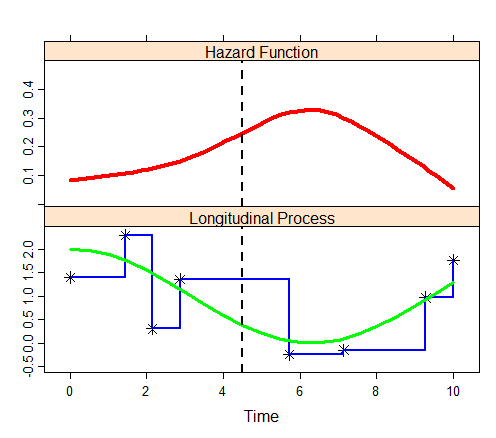
\includegraphics[scale=0.3]{JMidea.png}
\caption{Correlation between time-to-event outcome and longitudinal outcome (Rizopoulos, 2014 online)}
\end{figure}
\end{center}
 \end{itemize}
 
 
}



\frame{\frametitle{Background (Cont'd)}

\begin{itemize}
%\item Patients with hypertension are more likely to have heart failure related mortality and are then lost follow-up due to the events, which is called informative missing statistically. On the other side, the longitudinal measures of blood pressure can be an important predictor for heart failure events.

%\item When conducting data analysis with respect to either the longitudinal or time-to-event outcome, simply ignoring the correlation between them and fitting two models separately will lead to loss of information and misleading results.
%
%\item The linear mixed model (LMM), conventionally used for modeling longitudinal data, faces some challenges in applications such as it's sensitive to outliers and the conditional mean of the outcome may not be of research interest (Koenker 2005, Farcomeni 2014).
%
%\item Prediction of future event probabilities attracts great interest; joint modeling provides a great framework for such predictions. 

\item The joint modeling method: handle two types of data simultaneously
\item Linear mixed model (LMM) for longitudinal data
\begin{itemize}
\item Normality assumption may be invalid
\item Sensitive to outliers
\item Modeling conditional mean is not very meaningful from clinical perspective
\end{itemize}
\item Subject-specific predictions of event probabilities using joint modeling
\end{itemize} 
 
}






\subsection{Review of joint modeling} %%%%%%%


\frame{\frametitle{Joint modeling: When to use it? }
\begin{itemize}
\item When the focus is on the time-to-event outcome with {\bf time-varying covariate} measured with error
\item When the focus is on the longitudinal outcome and we would like to adjust for {\bf non-random} drop-outs 
\end{itemize}
  }



%\frame{\frametitle{Joint modeling: What is it?}
% 
%\begin{itemize}
%\item A set of two models, one for longitudinal process and the other for time-to-event process
%
%\item In the longitudinal process, the outcome variable consists of repeated measures taken from subjects followed over time
%
%\item In the time-to-event process, the outcome is the time until a specific event of interest occurs for the same group of subjects.
%
%\item The longitudinal outcome is a endogenous time-varying covariate in the time-to-event model
%
%\end{itemize}
% 
% 
%  }



\frame{\frametitle{Joint modeling: What is it?}


\small{
\begin{equation}\label{eqn:joint1}
\left\{
\begin{array}{l}
Y_{it} =m_{i}(t)+\varepsilon_{it}= {\boldsymbol X}_{it}^{\top}\boldsymbol{\beta} + {\boldsymbol Z}_{it}^{\top}{\boldsymbol u}_i + \varepsilon_{it}, \varepsilon_{it}\sim N(0, \sigma^2)\\
h(T_i|\mathcal{M}_{iT_i}, {\boldsymbol W}_i;  \boldsymbol{\gamma}, \alpha_1, 
\alpha_2) = h_0(T_i)\exp({\boldsymbol W}_i^{\top}\boldsymbol{\gamma} + \alpha m_{i}(T_i))
\end{array}
\right.
\end{equation}
}

\begin{itemize}
\item $Y_{it}$: the observed longitudinal outcome for $i$th subject at time $t$

%Specifically, let $Y_{it}$ be the longitudinal outcome for $i$th subject measured at time $t$ and let $T_i=\min(T_i^*, C_i)$ be the event time for the same subject, where $T_i^*$ is the true underlying event time and $C_i$ is the censoring time. The joint model can be formulated, in general, as
\item $T_i=\min(T_i^*, C_i)$: the event time for subject $i$, where $T_i^*$ is the true underlying event time and $C_i$ is the censoring time
\item $m_i(t)$: the error-free longitudinal measure; $\mathcal{M}_{iT_i}=\{m_i(s): 0\le s\le T_i\}$
\item $\boldsymbol{\beta}, \boldsymbol{\gamma}$: the fixed effects
\item $\boldsymbol{u}_i$: a vector of random effects for subject $i$
\item $\alpha$: the parameter governing the strength of association
\end{itemize}
  }


%\frame{\frametitle{Joint modeling: How to do it? }
% 
%\begin{itemize}
%\item Maximum likelihood estimation (MLE)\\\vspace{0.5em}
%
%Observed likelihood function:
%\end{itemize}
%
%
%\begin{eqnarray}\label{eqn:obs_likli}
%L(\boldsymbol{\theta};\boldsymbol{T,\Delta, Y})&=&\prod_{i=1}^N\int f(\boldsymbol{Y}_i|\boldsymbol{u}_i;\boldsymbol{\theta})f(T_i, \Delta_i|\boldsymbol{u}_i;\boldsymbol{\theta})f(\boldsymbol{u}_i;\boldsymbol{\theta})d\boldsymbol{u}_i\nonumber\\
%&=&\prod_{i=1}^N\int \prod_{t=1}^{n_i} f(Y_{it}|\boldsymbol{u}_i;\boldsymbol{\theta})f(T_i, \Delta_i|\boldsymbol{u}_i;\boldsymbol{\theta})f(\boldsymbol{u}_i;\boldsymbol{\theta})d\boldsymbol{u}_i
%\end{eqnarray}
%
%\begin{itemize}
%\item $\Delta_i$: event indicator (1 = death, 0 = censored)
%\item Numerical integration methods such as Monte Carlo and Gaussian quadrature
%\item Laplace approximation for high-dimensional random effects
%\end{itemize} 
% 
%  }
  
 
%\frame{\frametitle{Joint modeling: How to do it? (Cont'd)}
%
%%where \[f(T_i, \Delta_i|\boldsymbol{u}_i;\boldsymbol{\theta})=h(T_i|\mathcal{M}_{i}(T_i), \boldsymbol{W}_i;\boldsymbol{\theta})^{\Delta_i}S(T_i|\mathcal{M}_{i}(T_i), \boldsymbol{W}_i;\boldsymbol{\theta})^{1-\Delta_i},\]
%%\[S(T_i|\mathcal{M}_{i}(T_i), \boldsymbol{W}_i;\boldsymbol{\theta})=\exp\left\{-\int_0^{T_i} h(s|\mathcal{M}_{i}(s), \boldsymbol{W}_i;\boldsymbol{\theta})ds\right\},\]
%%\[\mathcal{M}_{i}(t) = \{m_{i}(s): 0\le s\le t\},\]
%%and  $h(\cdot)$ is given in (\ref{eqn:joint1}) the second equation.\\\vspace{0.5em}
%
%
%%Maximization of the log-likelihood is challenging due to the integration of random effects in (\ref{eqn:obs_likli}) as well as the integration in the definition of the survival function, but it can be done by using numerical integration methods such as Monte Carlo and Gaussian quadrature. For high-dimensional random effects, Laplace approximation can be useful.
%To obtain the MLE:
%\begin{itemize}
%\item Numerical integration methods such as Monte Carlo and Gaussian quadrature
%\item Laplace approximation for high-dimensional random effects
%\end{itemize} 
%}

\frame{\frametitle{Joint modeling: How to do it?}
\begin{itemize}
\item Bayesian method\\\vspace{0.5em}
Complete likelihood function:


\begin{eqnarray}\label{eqn:comp_likli}
L(\boldsymbol{\theta};\boldsymbol{T,\Delta, Y, u_i})&=&\prod_{i=1}^N f(\boldsymbol{Y}_i|\boldsymbol{u}_i;\boldsymbol{\theta})f(T_i, \Delta_i|\boldsymbol{u}_i;\boldsymbol{\theta})f(\boldsymbol{u}_i;\boldsymbol{\theta})\nonumber\\
&=&\prod_{i=1}^N \prod_{t=1}^{n_i} f(Y_{it}|\boldsymbol{u}_i;\boldsymbol{\theta})f(T_i, \Delta_i|\boldsymbol{u}_i;\boldsymbol{\theta})f(\boldsymbol{u}_i;\boldsymbol{\theta})
\end{eqnarray}

Next: derive the full conditional of each parameter.

\end{itemize}
  }


%\frame{\frametitle{Joint modeling: How to do it? (Cont'd)}
% 
%And the posterior distribution is given by 
%
%\begin{equation}\label{eqn:posterior}
%f(\boldsymbol{\theta}|\boldsymbol{T,\Delta, Y, u})\propto \prod_{i=1}^N \prod_{t=1}^{n_i} f(Y_{it}|\boldsymbol{u}_i;\boldsymbol{\theta})f(T_i, \Delta_i|\boldsymbol{u}_i;\boldsymbol{\theta})f(\boldsymbol{u}_i;\boldsymbol{\theta})\times f(\boldsymbol{\theta})
%\end{equation}
% where $f(\boldsymbol{\theta})$ is the prior distribution.
% 
%  }

  

\subsection{Review of quantile regression} %%%%%%%
\frame{\frametitle{Quantile Regression (QR)}
 {
\begin{itemize}
\item The $\tau$th quantile of a random variable $Y$, where $\tau\in[0,1]$
\begin{equation}\label{eqn:quantile}
Q_{Y}(\tau)=F_{Y}^{-1}(\tau)=\inf\left\{ y:Pr(Y\le y)\geq\tau\right\}
\end{equation}

\item QR models%s a specific quantile of the outcome as a linear function of the covariates:
\begin{equation}\label{eqn:lqr}
Q_{Y|{\boldsymbol X}}(\tau)={\boldsymbol X}^{\top}\boldsymbol{\beta}
\end{equation}
 
\item Inference method: 

\begin{equation}\label{eqn:loss_fun}
\hat{\boldsymbol{\beta}}_{\tau}=\underset{\boldsymbol{\beta}\in \mathbb{R}^{p}}{\mbox{arg min}}\sum_{i=1}^{n}\left[\rho_{\tau}(Y_{i}-{\boldsymbol X}_i^{\top}\boldsymbol{\beta})\right],
\end{equation}
where $\rho_{\tau}(Y)=Y(\tau-{I}{(Y<0)}).$
%\item There is no direct solution for Equation (\ref{eqn:loss_fun}), and linear programming method can be used to solve it. 
\end{itemize}
 }
  } 
 
\frame{\frametitle{Quantile Regression (QR) (Cont'd)}

\begin{center}
\begin{figure}
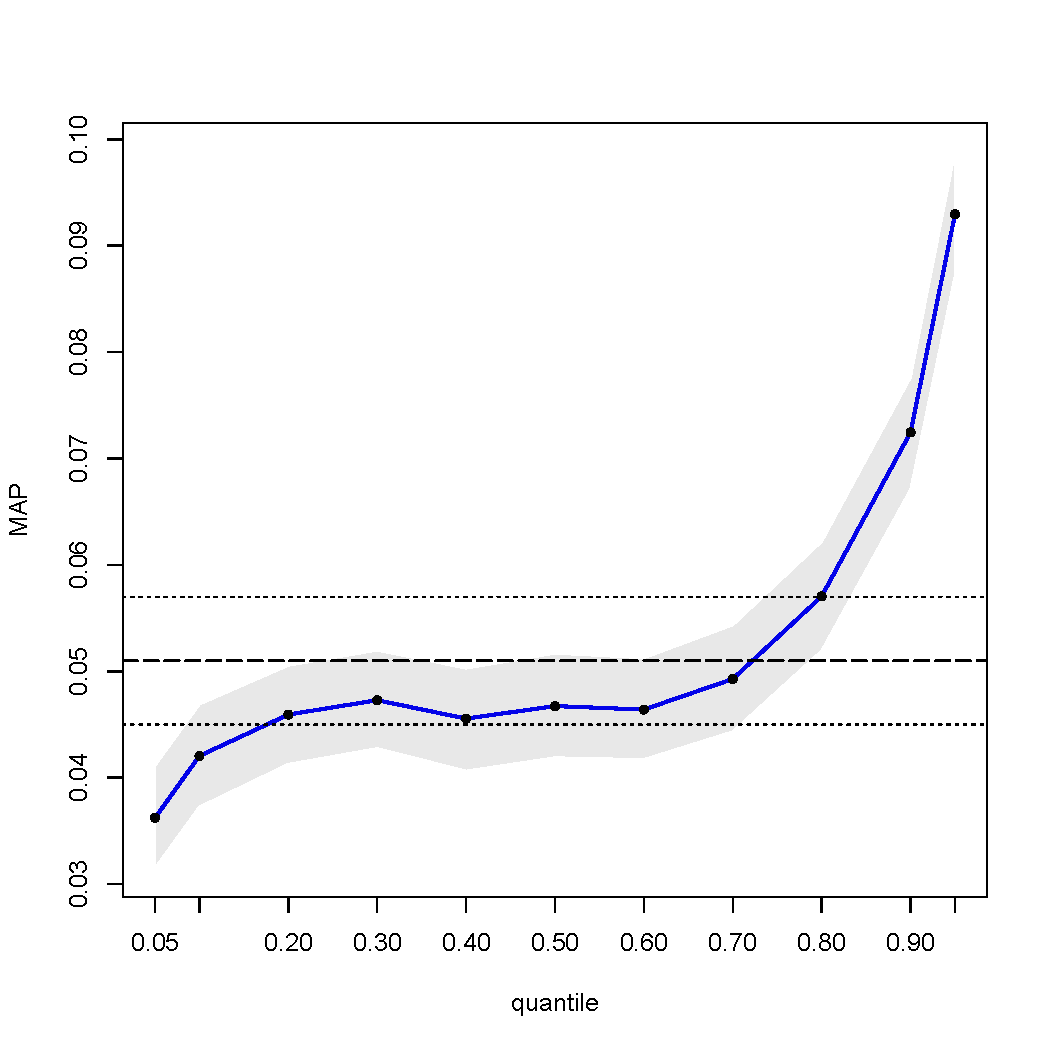
\includegraphics[scale=0.45]{MAP.pdf}
\caption{Quantile regression v.s. mean regression}
\end{figure}
\end{center}


}  
  
  

\frame{\frametitle{Asymmetric Laplace distribution (ALD)}
\small{
\begin{itemize}

\item Previous minimization problem can also be rephased as a maximum-likelihood problem by using ALD. 
\item An ALD is given by  

\begin{equation}\label{eqn:ald}
f(Y|\mu, \sigma, \tau)=\frac{\tau(1-\tau)}{\sigma}\exp\left[-\rho_{\tau}\left(\frac{Y-\mu}{\sigma}\right)\right],
\end{equation}

where $\mu\in(-\infty, \infty)$ is the location parameter, $\sigma$ is the scale parameter and $\tau\in(0, 1)$ is the skewness parameter. 

\begin{center}
\begin{figure}
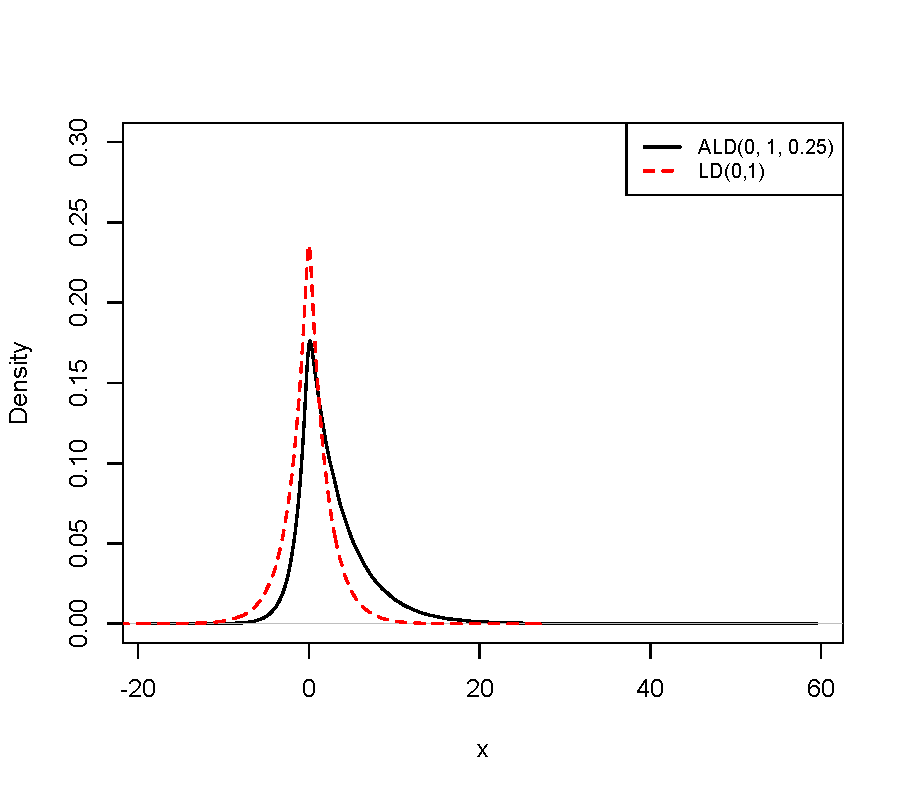
\includegraphics[scale=0.35]{ald_ld.pdf}\vspace{-2pt}
\caption{Asymmetric Laplace distribution and Laplace distribution}
\end{figure}
\end{center}

\end{itemize}
 }
  }
 


\frame{\frametitle{What have been done so far?}
\begin{itemize}
\item $\cdots$
%\item Fully Bayesian method to fit the JM using MCMC methods (Guo and Carlin, 2004)
%\item Multiple longitudinal outcomes (Brown et al., 2005; Rizopoulos and Ghosh, 2011); incorporating multiple failure times (Elashoff et al., 2008)
\item Make predictions of survival probabilities under the traditional JM framework (Rizopoulos, 2011) (Taylor et al., 2013)
\item Statistical inference of JM using quantile regression model for the longitudinal process (Farcomeni and Viviani, 2014)
\end{itemize} 

 
  }  

  
\subsection{Specific research aims} %%%%%%%
\frame{\frametitle{Specific research aim 1}


%\begin{enumerate}
\Large{ To develop a fully Bayesian method for subject-specific dynamic predictions of survival probabilities using quantile regression.}
%\end{enumerate}

 
  }
  
  
\frame{\frametitle{Specific research aim 2}

\Large {To extend Aim 1 to recurrent events data and obtain statistical inference.}

  }
  

\frame{\frametitle{Specific research aim 3}
 
\Large{ To extend Aim 2 to obtain subject-specific predictions of recurrent events probabilities.}

  }
  
  
 
\subsection{Public health significance} %%%%%%%
\frame{\frametitle{Public health significance}

\begin{itemize}

\item Using quantile regression to focus on the {\bf low or high tail} of the longitudinal outcome, which can be of greater interest clinically and more relevant to research questions 
\begin{itemize}
\item CD4 cell counts in HIV research (lower tail)
\item Study of low birth weight infants (lower tail)
\item hypertension in cardiovascular study (upper tail)
\item Prostate-Specific Antigen (PSA) levels in prostate cancer patients (upper tail)
\end{itemize}

\item Subject-specific predictions and healthcare
\begin{itemize}
\item The idea of "personalized medicine": to provide the right patient with the right drug at the right time
\item  Targeted treatment will be more subject specific thus more effective
\end{itemize}

%\item There is no Bayesian method developed yet for JM framework using quantile regression model
%\item Current JM prediction methods are all based on LMM but not quantile linear mixed model (QLMM).

\end{itemize}

  }


\frame{\frametitle{Public health significance (Cont'd)}
\begin{itemize}
\item Medicine revolution: from reactive to preventive
\item Enable the selection of optimal therapy
\item Assess individual drug response: reduce adverse drug reactions
\end{itemize}

\begin{center}
\begin{figure}
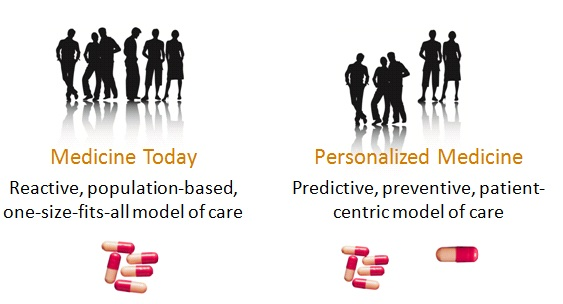
\includegraphics[scale=0.7]{per_med.jpg}
%\caption{Example of subject-specific dynamic predictions for survival probabilities (Rizopoulos, 2011)}
\end{figure}
\end{center}

  }
  



%%%%%%%%%%%%%%%%%==METHODS==%%%%%%%%%%%%%%%%%%%%%%%% 
\section{Statistical methods} %%%%%%%
\frame{\frametitle{Statistical methods}

\begin{itemize}
\item JM using longitudinal quantile regression
\item Subject-specific dynamic predictions 
\item Predictive performance of longitudinal biomarker
\end{itemize}
 
}
  
  
 


\subsection{JM using longitudinal quantile regression} %%%%%%%
\frame{\frametitle{Longitudinal quantile regression}

\begin{itemize}
\item The linear quantile mixed model (LQMM):
\begin{equation}\label{eqn:lqmm}
Q_{Y_{ij}|{\boldsymbol X}_{ij},{\boldsymbol Z}_{ij}}(\tau)={\boldsymbol X}_{ij}^{\top} \boldsymbol{\beta}_{\tau}+ {\boldsymbol Z}_{ij}^{\top}\boldsymbol{u}_i,\ i=1, \cdots, N;\ j=1,\cdots, n_i.
\end{equation}

%{\small where $Y_{ij}$ is the outcome for subject $i$ at time $j$, ${\boldsymbol X}_{ij}$ is the $p-$dimensional fixed effects covariates and $\boldsymbol{\beta}_{\tau}$ is the corresponding $p\times1$ vector of fixed effects, while ${\boldsymbol Z}_{ij}$ is the $k-$dimensional random effects covariates and $\boldsymbol{u}_i$ is the corresponding $k\times 1$ vector of random effects for subject $i$.}


\item Under $\varepsilon_{ij}\sim $ ALD$(0, \sigma, \tau)$, $Y_{ij}|\boldsymbol{u}_i\overset{iid}\sim$ ALD(${\boldsymbol X}_{ij}^{\top}\boldsymbol{\beta}+{\boldsymbol Z}_{ij}^{\top}\boldsymbol{u}_i, \sigma, \tau$):

\begin{equation}\label{eqn:ald_lqmm}
f(Y_{ij}|\boldsymbol{u}_i;\boldsymbol{\beta}_{\tau},\sigma)=\frac{\tau(1-\tau)}{\sigma}\exp\left[-\rho_{\tau}\left(\frac{Y_{ij}-{\boldsymbol X}_{ij}^{\top}\boldsymbol{\beta}-{\boldsymbol Z}_{ij}^{\top}\boldsymbol{u}_i}{\sigma}\right)\right]
\end{equation}

\end{itemize} 
  } 
  
  
\frame{\frametitle{Longitudinal quantile regression (Cont'd)}

\begin{itemize}
\item The location-scale mixture representation of the ALD (Kotz et al., 2001):

\[\varepsilon_{ij}=\kappa_1e_{ij}+\kappa_2\sqrt{\sigma e_{ij}}v_{ij}.\]

\begin{equation}\label{eqn:reformald2}
Y_{ij}={\boldsymbol X}_{ij}^{\top}\boldsymbol{\beta}+{\boldsymbol Z}_{ij}^{\top}\boldsymbol{u}_i+\kappa_1e_{ij}+\kappa_2\sqrt{\sigma e_{ij}}v_{ij}.
\end{equation}


where 

\[\kappa_1=\frac{1-2\tau}{\tau(1-\tau)}, \kappa_2^2=\frac{2}{\tau(1-\tau)},\]
and \[v_{ij}\sim N(0,1), e_{ij}\sim\exp(1/\sigma).\]

\end{itemize} 
  }  
  

\frame{\frametitle{Longitudinal quantile regression and JM}

%\begin{itemize}
%\item A new version of JM is then developed by replacing the conventional linear mixed model (LMM) with the longitudinal QR.
%
%\item Specifically, in our study we will use the following JM

\begin{equation}\label{eqn:joint}
\left\{
\begin{array}{l}
Y_{it} = {\boldsymbol X}_{it}^{\top}\boldsymbol{\beta} + {\boldsymbol H}_{it}^{\top}\boldsymbol{\delta} + {\boldsymbol Z}_{it}^{\top}{\boldsymbol u}_i + \varepsilon_{it}, \varepsilon_{it}\sim ALD(0, \sigma,\tau)\\
h(T_i|\mathcal{M}_{iT_i}, {\boldsymbol W}_i;  \boldsymbol{\gamma}, \alpha_1, 
\alpha_2) = h_0(T_i)\exp({\boldsymbol W}_i^{\top}\boldsymbol{\gamma} + \alpha_1{\boldsymbol H}_{iT_i}^{\top}\boldsymbol{\delta} + \alpha_2{\boldsymbol Z}_{iT_i}^{\top}{\boldsymbol u}_{i})
\end{array}
\right.
\end{equation}

Example: 
\begin{itemize}
\item $\boldsymbol{Y}$: Left ventricular ejection fraction (LVEF)
\item $\boldsymbol{T}$: Time to death
\item $\boldsymbol{X}$: intercept and age
\item $\boldsymbol{H}$: mildly dilated cardiomyopathy (MDCM) indicator $\times$ $(1\hspace{1em} t)$
\item $\boldsymbol{W}$: gender, New York Heart Association (HYHA) functional class
\item $\boldsymbol{Z}$: $(1\hspace{1em}  t)$
\end{itemize}

%\item {\small $\boldsymbol{X}_{it}$ and $\boldsymbol{H}_{it}$ are the fixed effects covariates that are associated with the outcome and $\boldsymbol{Z}_{it}$ are the covariates associated with $k-$dimensional random effects $\boldsymbol{u}_i$;}
%
%\item{\small $\boldsymbol{W}_{i}$ are the fixed effects covariates that are only associated with event time (not longitudinal outcome) and this model shares the same fixed effects covariates $\boldsymbol{H}_{it}$ and random effects covariates $\boldsymbol{Z}_{it}$ with the longitudinal model. }

%\item {\small The two models are related by sharing some of the fixed and random variables, and the degree of associations from those two sources of measurements (observed and unobserved) are measured by another two parameters $\alpha_1$ and $\alpha_2$, respectively.}


%\end{itemize} 
  } 
  
  
%\frame{\frametitle{Model estimation}
%\begin{itemize}
%\item Under the location-scale mixture representation of the longitudinal QR model, in (\ref{eqn:joint})
%\[
%Y_{it}|\boldsymbol{u}_i \overset{iid}\sim N({\boldsymbol X}_{it}^{\top}\boldsymbol{\beta} + {\boldsymbol H}_{it}^{\top}\boldsymbol{\delta} + {\boldsymbol Z}_{it}^{\top}{\boldsymbol u}_i+\kappa_1e_{ij}, \kappa_2^2\sigma e_{ij})
%\]
%
%\item The survival likelihood is given by 
%\[f(T_i, \Delta_i|\boldsymbol{u}_i;\boldsymbol{\theta})=h(T_i|\mathcal{M}_{i}(T_i), \boldsymbol{W}_i;\boldsymbol{\theta})^{\Delta_i}S(T_i|\mathcal{M}_{i}(T_i), \boldsymbol{W}_i;\boldsymbol{\theta})^{1-\Delta_i},\] where 
%$S(T_i|\mathcal{M}_{i}(T_i), \boldsymbol{W}_i;\boldsymbol{\theta})=\exp\left\{-\int_0^{T_i} h(s|\mathcal{M}_{i}(s), \boldsymbol{W}_i;\boldsymbol{\theta})ds\right\},$
%and  $h(\cdot)$ is given in (\ref{eqn:joint}) the second equation.\\\vspace{0.5em}
%
%\item The complete likelihood is given in (\ref{eqn:comp_likli}); and we can then apply the Gibbs sampler to get the parameter estimation.
%
%\end{itemize}
%
%}



\subsection{Dynamic predictions of event probabilities}%%%%%%%%%%
\frame{\frametitle{Dynamic predictions of future event probabilities}

\begin{itemize}
\item Notations:
\begin{itemize}
\item $\mathcal{Y}_i(t)=\{Y_i(s), 0\le s\le t\}$: complete history of observed longitudinal outcome for patient $i$ up to time $t$ 
\item $\mathcal{D}_n=\{T_i, \Delta_i, \boldsymbol{Y}_i, i=1, \cdots, n\}$: the training data
\item $p_i(m|t) = Pr(T_i^*\ge m|T_i^*>t, \mathcal{Y}_i(t), \mathcal{D}_n;\boldsymbol{\theta})$: the probability that patient $i$ is free of event up to time $m>t$, given he/she is free of event until time $t$.
\end{itemize}

\item The predicted probability of no event until time $m$ is then given by 

{\small 
\begin{eqnarray}\label{eqn:surv_prob_derv}
&&\nonumber Pr(T_i^*\ge m|T_i^*>t, \mathcal{Y}_i(t), \mathcal{D}_n;\boldsymbol{\theta})\\
%&=&\nonumber\int Pr(T_i^*\ge m|T_i^*>t, \mathcal{Y}_i(t), \mathcal{D}_n, u_i;\boldsymbol{\theta})\times Pr(u_i|T_i^*>t, \mathcal{Y}_i(t), \mathcal{D}_n;\boldsymbol{\theta})du_i\\
%\nonumber&=&\int Pr(T_i^*\ge m|T_i^*>t, u_i;\boldsymbol{\theta})Pr(u_i|T_i^*>t, \mathcal{Y}_i(t);\boldsymbol{\theta})du_i\\
&=&\int\frac{{S}_i[m|\mathcal{M}_i(m, u_i, \boldsymbol{\theta});\boldsymbol{\theta}]}{{S}_i[t|\mathcal{M}_i(t, u_i, \boldsymbol{\theta});\boldsymbol{\theta}]}Pr(u_i|T_i^*>t, \mathcal{Y}_i(t);\boldsymbol{\theta})du_i,
\end{eqnarray}
}
\end{itemize}
 
  } 


\frame{\frametitle{Dynamic predictions of future event probabilities (Cont'd)}
{\small 
\begin{itemize}
%\item We may approximate (\ref{eqn:surv_prob_derv}) by using the MCMC algorithm. Specifically the posterior expectation of it
%
%\begin{eqnarray}\label{eqn:expct_pred}
%\nonumber E_{\boldsymbol{\theta}|\mathcal{D}_n}[p_i(m|t)]&=&Pr(T_i^*\ge m|T_i^*>t, \mathcal{Y}_i(t), \mathcal{D}_n)\\
%&=&\int Pr(T_i^*\ge m|T_i^*>t, \mathcal{Y}_i(t);\boldsymbol{\theta})p(\boldsymbol{\theta}|\mathcal{D}_n)d\boldsymbol{\theta}.
%\end{eqnarray}

\item Monte Carlo (MC) estimate of $p_i(m|t)$: %upon collecting all of the $K$ samples, the value of $p_i(m|t)$ can be calculated as the sample mean or median and the standard error can be computed using the sample variance.

%\begin{algorithm}[H]
%\caption{MC algorithm to draw samples of $p_i(m|t)$}\label{draw_pi}
%\begin{algorithmic}
%\For{$k$ in $1:K$} 
%\State draw $\boldsymbol{\theta}^{(k)}\sim f(\boldsymbol{\theta}|\mathcal{D}_n)$
%\State draw $u^{(k)}_i\sim f(u_i|T_i^*>t, \mathcal{Y}_i(t), \boldsymbol{\theta}^{(k)})$
%\State compute $p_i^{(k)}(m|t)=S_i[m|\mathcal{M}_i(m, u^{(k)}_i, \boldsymbol{\theta}^{(k)});\boldsymbol{\theta}^{(k)}]S_i[t|\mathcal{M}_i(t, u^{(k)}_i, \boldsymbol{\theta}^{(k)});\boldsymbol{\theta}^{(k)}]^{-1}$
%\EndFor
%\end{algorithmic}
%\end{algorithm}
\begin{itemize}
\item draw $\boldsymbol{\theta}^{(k)}\sim f(\boldsymbol{\theta}|\mathcal{D}_n)$;
\item draw $u^{(k)}_i\sim f(u_i|T_i^*>t, \mathcal{Y}_i(t), \boldsymbol{\theta}^{(k)})$
\item compute $p_i^{(k)}(m|t)=S_i[m|\mathcal{M}_i(m, u^{(k)}_i, \boldsymbol{\theta}^{(k)});\boldsymbol{\theta}^{(k)}]S_i[t|\mathcal{M}_i(t, u^{(k)}_i, \boldsymbol{\theta}^{(k)});\boldsymbol{\theta}^{(k)}]^{-1}$
\end{itemize}

\item Sample mean or median:
\begin{equation}\label{eqn:sample_mean}
\hat{p}_i(m|t)=\frac{1}{K}\sum_{k=1}^K p^{(k)}_i(m|t),
\end{equation}

\end{itemize}
} 
  } 
  
  
  
\frame{\frametitle{Dynamic predictions of future event probabilities (Cont'd)}

\begin{center}
\begin{figure}
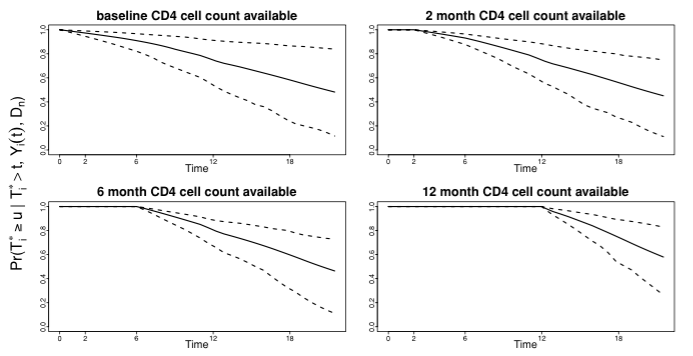
\includegraphics[scale=0.45]{prediction.png}
\caption{Example of subject-specific dynamic predictions for survival probabilities (Rizopoulos, 2011)}
\end{figure}
\end{center}

  } 
  


\subsection{Predictive performance of the longitudinal biomarker} %%%%%%%
\frame{\frametitle{Predictive performance of the longitudinal biomarker}
%Here we focus on the predictive ability of the longitudinal outcome in terms of how well the model discriminate patients who will have event from those who will not.

\begin{itemize}


\item Sensitivity
\begin{equation}\label{eqn:sensitivity}
Pr[\mathcal{S}_i(k,t, \boldsymbol{c})|T_i^*>t, T_i^*\in (t, t+\Delta t];\boldsymbol{\theta}]
\end{equation}

\item Specificity
\begin{equation}\label{eqn:specificity}
Pr[\mathcal{F}_i(k,t, \boldsymbol{c})|T_i^*>t, T_i^* > t+\Delta t;\boldsymbol{\theta}]
\end{equation}

\item Notations: 
\begin{itemize}
\item $\mathcal{S}_i(k,t, {\boldsymbol c})=\{Y_i(s)\le c_s, k\le s\le t\}$ is defined as success (or event) 
\item $\mathcal{F}_i(k,t, \boldsymbol{c})=\mathbb{R}^{n(k,t)}\setminus\{Y_i(s)\le c_s, k\le s\le t\}$ is defined as failure
\item $\boldsymbol{c}$ is a vector of threshold values and $c_s$ is the threshold value at time $s$
\item $\mathbb{R}^n$ denotes the $n-$dimensional Euclidean space
\item $n(k,t)$ is the total number of longitudinal measurements in interval $[k,t]$
\end{itemize}


\end{itemize}
  } 

    
%\frame{\frametitle{Predictive performance of the longitudinal biomarker (Cont'd)}
%
%\begin{itemize}
%\item Derivation of the sensitivity
%{\small
%\begin{eqnarray*}
%&&Pr\{\mathcal{S}_i(t,k,\boldsymbol{c})|T_i^*>t, T_i^*\in (t, t+\Delta t]\}=\frac{Pr\{\mathcal{S}_i(t,k,\boldsymbol{c}),T_i^*\in (t, t+\Delta t]|T_i^*>t\}}{1- Pr(T_i^* > t+\Delta t|T_i^*>t)}
%\end{eqnarray*}
%}
%
%\item The numerator 
%{\small
%\begin{eqnarray}\label{eqn:sen_num}
%\nonumber && Pr\{\mathcal{S}_i(t,k,\boldsymbol{c}),T_i^*\in (t, t+\Delta t]|T_i^*>t\}\\
%&=&\nonumber\int Pr\{\mathcal{S}_i(t,k,\boldsymbol{c}),T_i^*\in (t, t+\Delta t]|T_i^*>t, u_i\}\times p(u_i|T^*_i>t)du_i\\
%\nonumber &=&\int\left\{\prod_{s=k}^t\Phi\left[\frac{c_s-\omega_i(s)}{\xi}\right]\right\}\\
%&\times&\left[1-\frac{\mathcal{S}_i\{t+\Delta t|\mathcal{M}_i(t+\Delta t, u_i)\}}{\mathcal{S}_i\{t|\mathcal{M}_i(t,u_i)\}}\right]\times p(u_i|T^*_i>t)du_i
%\end{eqnarray}
%}
%
%
%\item The denominator
%{\small
%\begin{eqnarray}
%1-Pr(T_i^* > t+\Delta t|T_i^*>t)=1-\int\frac{\mathcal{S}_i\{t+\Delta t|\mathcal{M}_i(t+\Delta t, u_i)\}}{\mathcal{S}_i\{t|\mathcal{M}_i(t,u_i)\}}p(u_i|T^*_i>t)du_i
%\end{eqnarray}
%}
%
%\end{itemize}
% } 
%  


%\frame{\frametitle{Predictive performance of the longitudinal biomarker (Cont'd)}
%
%\begin{itemize}
%\item Based on above derivations, we now can develop the following MC algorithm to simulate samples of the sensitivity:
%
%\begin{algorithm}[H]
%\caption{MC algorithm to compute sensitivity of the predictions}\label{draw_sensitivity}
%\begin{algorithmic}
%\For{$k$ in $1:K$} 
%\State draw $\boldsymbol{\theta}^{(k)}\sim f(\boldsymbol{\theta}|\mathcal{D}_n)$
%\State draw $\mathcal{Y}^{(k)}_i(t)\sim N({\boldsymbol X}_{it}^{\top}\boldsymbol{\beta}^{(k)} + {\boldsymbol H}_{it}^{\top}\boldsymbol{\delta}^{(k)} + {\boldsymbol Z}_{it}^{\top}{\boldsymbol u}_i^{(k-1)} + \kappa_1 e_{ij}, \kappa_2^2\sigma^{(k)} e_{ij} )$
%\State draw $u^{(k)}_i\sim f(u_i|T_i^*>t, \mathcal{Y}^{(k)}_i(t), \boldsymbol{\theta}^{(k)})$
%\State compute $\mathcal{E}_1(u_i^{(k)}, \boldsymbol{\theta}^{(k)})$ and $\mathcal{E}_2(u_i^{(k)}, \boldsymbol{\theta}^{(k)})$
%\EndFor
%\end{algorithmic}
%\end{algorithm}
%
%\item where $\mathcal{E}_1(u_i, \boldsymbol{\theta})=\left\{\prod_{s=k}^t\Phi\left[\frac{c_s-\omega_i(s)}{\xi}\right]\right\}\left[1-\frac{\mathcal{S}_i\{t+\Delta t|\mathcal{M}_i(t+\Delta t, u_i)\}}{\mathcal{S}_i\{t|\mathcal{M}_i(t,u_i)\}}\right]$ and $\mathcal{E}_2(u_i, \boldsymbol{\theta})=\mathcal{S}_i\{t+\Delta t|\mathcal{M}_i(t+\Delta t, u_i)\}\mathcal{S}_i\{t|\mathcal{M}_i(t,u_i)\}^{-1}$ and we can calculate the MC estimate of the sensitivity as follows:
%
%\begin{equation}\label{eqn:est_sensitivity}
%\widehat{Pr}[\mathcal{S}_i(t,k,\boldsymbol{c})|T_i^*>t, T_i^*\in (t, t+\Delta t];\boldsymbol{\theta}] =\frac{\sum_{k=1}^K\mathcal{E}_1(u_i^{(k)}, \boldsymbol{\theta}^{(k)})/K}{1-\sum_{k=1}^K\mathcal{E}_2(u_i^{(k)}, \boldsymbol{\theta}^{(k)})/K}.
%\end{equation}
%
%\end{itemize}
%
%  } 


  
\frame{\frametitle{Predictive performance of the longitudinal biomarker (Cont'd)}


\begin{center}
\begin{figure}
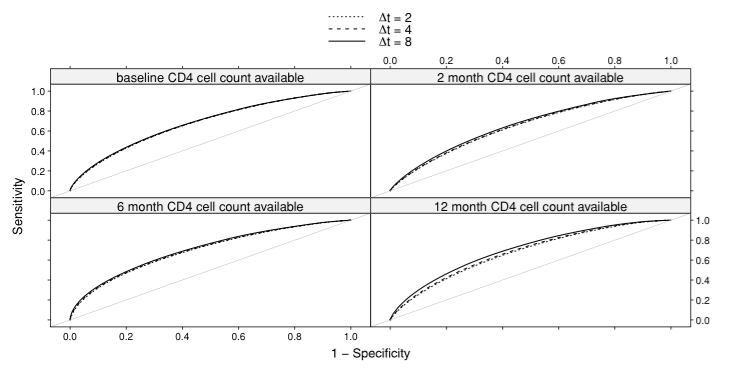
\includegraphics[scale=0.45]{validation.png}
\caption{Example of ROCs for predictive performance (Rizopoulos, 2011)}
\end{figure}
\end{center}

  } 



%%%%%%%%%%%%%%%%%==SIMULATION==%%%%%%%%%%%%%%%%%%%%%%%%
\section{Simulation studies} %%%%%%%
\frame{\frametitle{Simulation studies}
 
\begin{itemize}
\item {\bf Simulation Study 1}: validity of proposed Bayesian inference method
%The first simulation study is designed to to check the accuracy of our proposed fully Bayesian estimating algorithm, which is the crucial basis for future prediction performance. By varying the values of the association parameters $\alpha_1$ and $\alpha_2$ in our model (\ref{eqn:joint}), we will have four different settings for simulation study, which are:

\begin{enumerate}
\item $(\alpha_1, \alpha_2)=(0, 0)$, the two models are indepdent with each other
\item $(\alpha_1, \alpha_2)=(1, 0)$, the two models are related only through the observed heterogeneity in some covarites, i.e. ${\boldsymbol H}_{it}$ in our model
\item $(\alpha_1, \alpha_2)=(0, 1)$, the two models are related only through the unobserved heterogeneity, i.e. the random effects
\item $(\alpha_1, \alpha_2)=(1, 1)$, the depdence of the two models is explained by both observed and unobserved heterogeneity
\end{enumerate}

\end{itemize}

{\tiny 
\begin{table}[H]
\begin{center}
\caption{Bias and standard error of the parameter estimates from proposed fully Bayesian estimating method}
\begin{tabular}{ccccccccccccc}
\hline
\multicolumn{13}{c}{$\tau$=0.25}\\
\hline
&&&\multicolumn{2}{c}{${\beta}$}&\multicolumn{2}{c}{${\delta}$}&\multicolumn{2}{c}{${\gamma}$}&\multicolumn{2}{c}{$\alpha_1$}&\multicolumn{2}{c}{$\alpha_2$}\\
n & $\alpha_1$ & $\alpha_2$  & bias & s.d.& bias & s.d. & bias & s.d. & bias & s.d. & bias & s.d. \\
500 & 0 & 0 &   &   &   &   &   &   &   &   & 	&  \\
500 & 1 & 0 &   &   &   &   &   &   &   &   &   &  \\
500 & 0 & 1 & 	& 	& 	& 	& 	& 	& 	& 	& 	&  \\
500 & 1 & 1 & 	& 	& 	& 	& 	& 	&	& 	& 	&  \\
\hline
\end{tabular} 
\label{tab:sim1} 
\end{center}
\end{table}
}
} 
  


%%%%%%%%%%%%%%%%%==SIMULATION==%%%%%%%%%%%%%%%%%%%%%%%%
\frame{\frametitle{Simulation studies (Cont'd)}
{\small
\begin{itemize}
\item {\bf Simulation Study 2}: accuracy of the prediction method
%In this simulation study, we will use the true simulated random effects, covariates and coefficients to calculate the survival probability for subject $i$ as 

\item Statistics to be compared -- Equation (\ref{eqn:surv_prob_derv}):

\[\frac{S_i[m|\mathcal{M}_i(m, u_i, \boldsymbol{\theta});\boldsymbol{\theta}]}{S_i[t|\mathcal{M}_i(t, u_i, \boldsymbol{\theta});\boldsymbol{\theta}]}.\]

%\item We then use Algorithm \ref{draw_pi} to computed the predicted survival probability for the same subject. By doing this for many different selected subjects, we will be able to evaluate how "close" the predicted values from our proposed model are to the true values by using Bland-Altman plot (Bland and Altman, 1986).
\item  Compare the predicted values with the ''gold standard'', i.e. the simulated values

\end{itemize}
}
\small{
\begin{table}[H]
\resizebox{1\textwidth}{!}{
\begin{minipage}{1\textwidth}
\begin{center}
\begin{tabular}{cccc}
\hline
 & $\Delta t=2$ & $\Delta t=4$ &$\Delta t=6$ \\
 \hline
& bias(lower, upper) & bias(lower, upper) & bias(lower, upper)\\
$t$=2 &	&	&\\
$t$=4 &	&	&\\
$t$=8 &	&	&\\
$t$=16 &	&	&\\
\hline
\end{tabular}
\label{tab:sim2}
\caption{Summary table of comparing the predictive results from proposed method with gold standard}
\end{center}
\end{minipage} 
}
\end{table}
}
} 


\frame{\frametitle{Simulation plans (Cont'd)}

\begin{center}
\begin{figure}
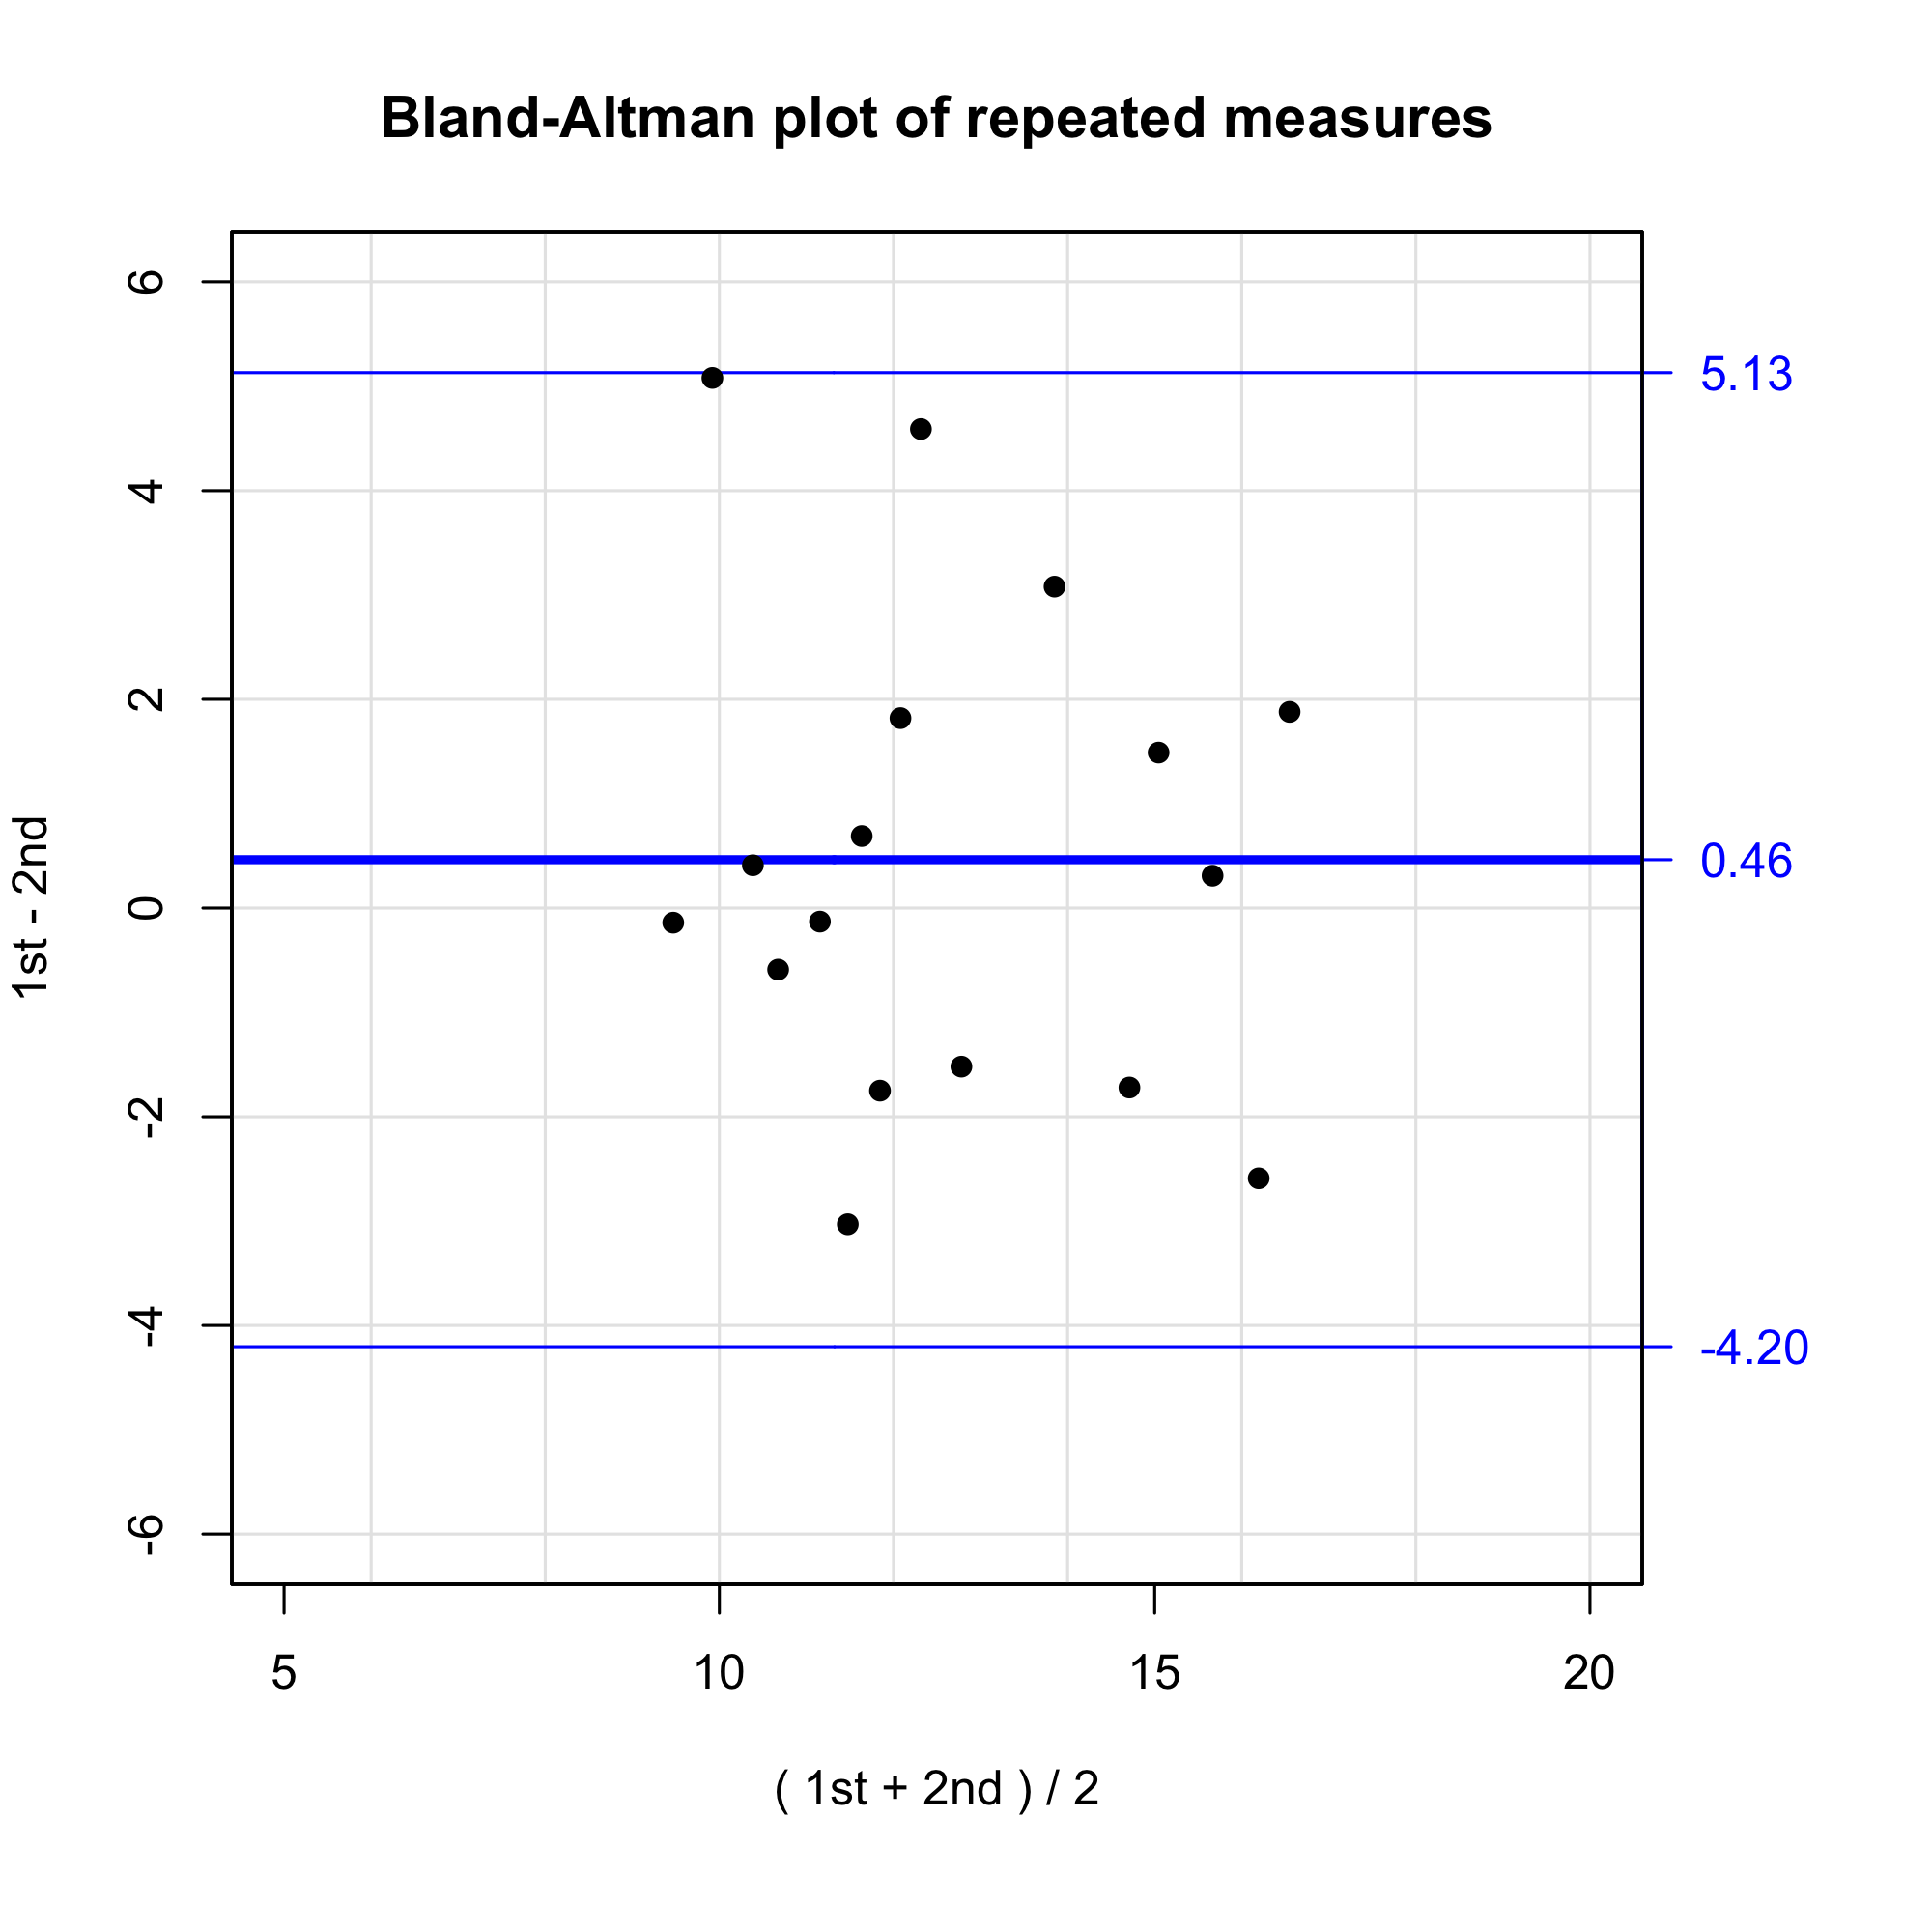
\includegraphics[scale=0.1]{ba_plot.png}
\caption{An example of Bland-Altman plot}
\end{figure}
\end{center}


} 





%%%%%%%%%%%%%%%%%==DATA==%%%%%%%%%%%%%%%%%%%%%%%%
 \section{Real data} %%%%%%%
\frame{\frametitle{Real data }

\begin{itemize}
\item The Antihypertensive and Lipid-Lowering Treatment to Prevent Heart Attack Trial (ALLHAT)  (1994-2002): multi-center, randomized, double-blind, active-controlled clinical trial. 

\item 42,448 participants, 625 sites. 

\item 19\% Hispanic patients, 46.8\% women, 67 years old on average (with 35\% aged $\ge$70 years), 36\% of patients with diabetes, 47\% are cardiovascular disease patients and 22\% are smokers.

\item Primary outcome: fatal coronary heart disease (CHD) or non-fatal myocardial infarction (MI)
\item Secondary endpoints: cardiovascular events (stroke, heart failure (HF), CHD, etc.). 
\end{itemize}
} 


\frame{\frametitle{Description of real data (Cont'd)}

\begin{center}
\begin{figure}
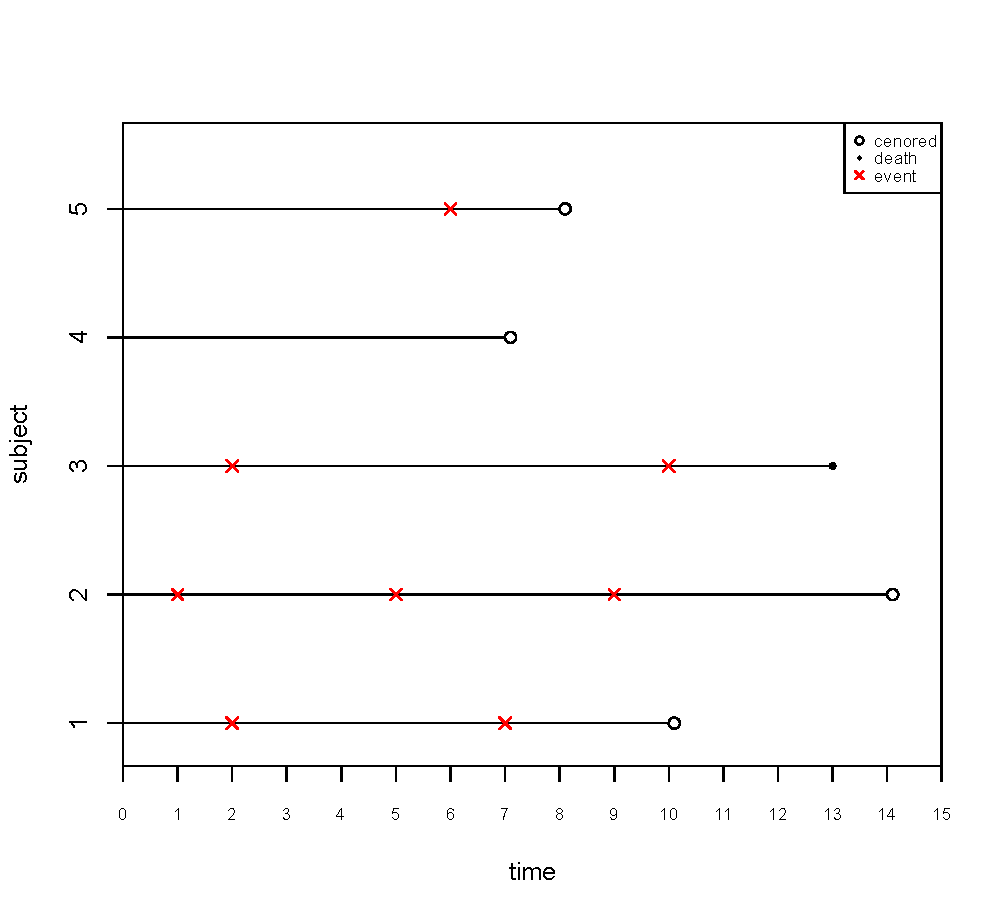
\includegraphics[scale=0.5]{recurrent_event.pdf}
\caption{An example of recurrent events (e.g. stroke) data}
\end{figure}
\end{center}


} 

  


%%%%%%%%%%%%%%%%%==Acknowledgement==%%%%%%%%%%%%%%%%%%%%%%%%
 \section{Acknowledgement} %%%%%%%
\frame{\frametitle{Acknowledgement}
\begin{itemize}
\item {\bf Dissertation committee:}

{Stacia M. DeSantis, PhD (Chair \& Academic Advisor)}\par\vspace{0.5em}
{Sheng Luo, PhD (Dissertation Supervisor)}\par\vspace{0.5em}
{David R. Lairson, PhD (Minor Adviosr)}\par\vspace{0.5em}
{Xiaoming Liu, PhD (Breadth Advisor)}\\

\vspace{1em}
\item{\bf Externel reviewer:}

{Soeun Kim, PhD}


\end{itemize}
 
} 
  



%%%%%%%%%%%%%%%%%==References==%%%%%%%%%%%%%%%%%%%%%%%%
 \section{References} %%%%%%%
\frame{\frametitle{Selected references}

\begin{thebibliography}{4}  


 \beamertemplatearticlebibitems
  \bibitem{bland1986statistical}
    J Martin Bland and Douglas G Altman
   \newblock Statistical methods for assessing agreement between two methods of clinical measurement.
    \newblock {\em The Lancet}, 327(8476):307--310, 1986.

 \beamertemplatearticlebibitems
  \bibitem{davis1996rationale}
    Barry R Davis, Jeffrey A Cutler, David J Gordon, Curt D Furberg, Jackson T Wright, William C Cushman, Richard H Grimm, John LaRosa, Paul K Whelton and H Mitchell Perry
    \newblock Rationale and design for the antihypertensive and lipid lowering treatment to prevent heart attack trial (ALLHAT).
    \newblock {\em American Journal of Hypertension}, 9(4):342--360, 1996.

    
 \beamertemplatearticlebibitems
  \bibitem{kotz2001laplace}
    Samuel Kotz, Tomasz Kozubowski and Krzysztof  Podgorski
    \newblock The Laplace Distribution and Generalizations: A Revisit With Applications to Communications, Exonomics, Engineering, and Finance.
    \newblock {\em Springer}, 2001.
    
%  \beamertemplatearticlebibitems
%  \bibitem{guo2004separate}
%    Xu Guo and Bradley P Carlin
%    \newblock Separate and joint modeling of longitudinal and event time data using standard computer packages
%    \newblock {\em The American Statistician}, 58(1):16--24, 2004.
%

    
  \end{thebibliography}      
}  





\frame{\frametitle{Selected references (Cont'd)}
\begin{thebibliography}{4}  

%  \beamertemplatearticlebibitems
%  \bibitem{brown2005flexible}
%    Elizabeth R Brown, Joseph G Ibrahim and Victor DeGruttola
%    \newblock A Flexible B-Spline Model for Multiple Longitudinal Biomarkers and Survival.
%    \newblock {\em Biometrics}, 61(1):64--73, 2005.

      
  \beamertemplatebookbibitems
  \bibitem{koenker2005quantile}
    Roger Koenker
    \newblock Quantile regression.
    \newblock {\em Cambridge university press}, 2005.

%  \beamertemplatearticlebibitems
%  \bibitem{elashoff2008joint}
%	Robert M Elashoff, Gang Li and Ning Li
%    \newblock A joint model for longitudinal measurements and survival data in the presence of multiple failure types.
%    \newblock {\em Biometrics}, 64(3):762--771, 2008.
    
  \beamertemplatearticlebibitems
  \bibitem{rizopoulos2011dynamic}
    Dimitris Rizopoulos
    \newblock Dynamic Predictions and Prospective Accuracy in Joint Models for Longitudinal and Time-to-Event Data.
    \newblock {\em Biometrics}, 67(3):819--829, 2011.
    
    
  \beamertemplatearticlebibitems
  \bibitem{taylor2013real}
   Jeremy MG Taylor, Yongseok Park, Donna P Ankerst, Cecile Proust-Lima, Scott Williams, Larry Kestin, Kyoungwha Bae, Tom Pickles and Howard Sandler
    \newblock Real-time individual predictions of prostate cancer recurrence using joint models.
    \newblock {\em Biometrics}, 69(1):206--213, 2013.
  
     
     
  \beamertemplatearticlebibitems
  \bibitem{Alessio2014qrjm}
    Alessio Farcomeni and Sara Viviani
    \newblock Longitudinal quantile regression in the presence of informative dropout through longitudinal--survival joint modeling.
    \newblock {\em Statistics in Medicine}, 2014.
  \end{thebibliography}
 

}  





    
\end{document}